\section{Motivating example}
\begin{figure}[h]
\center{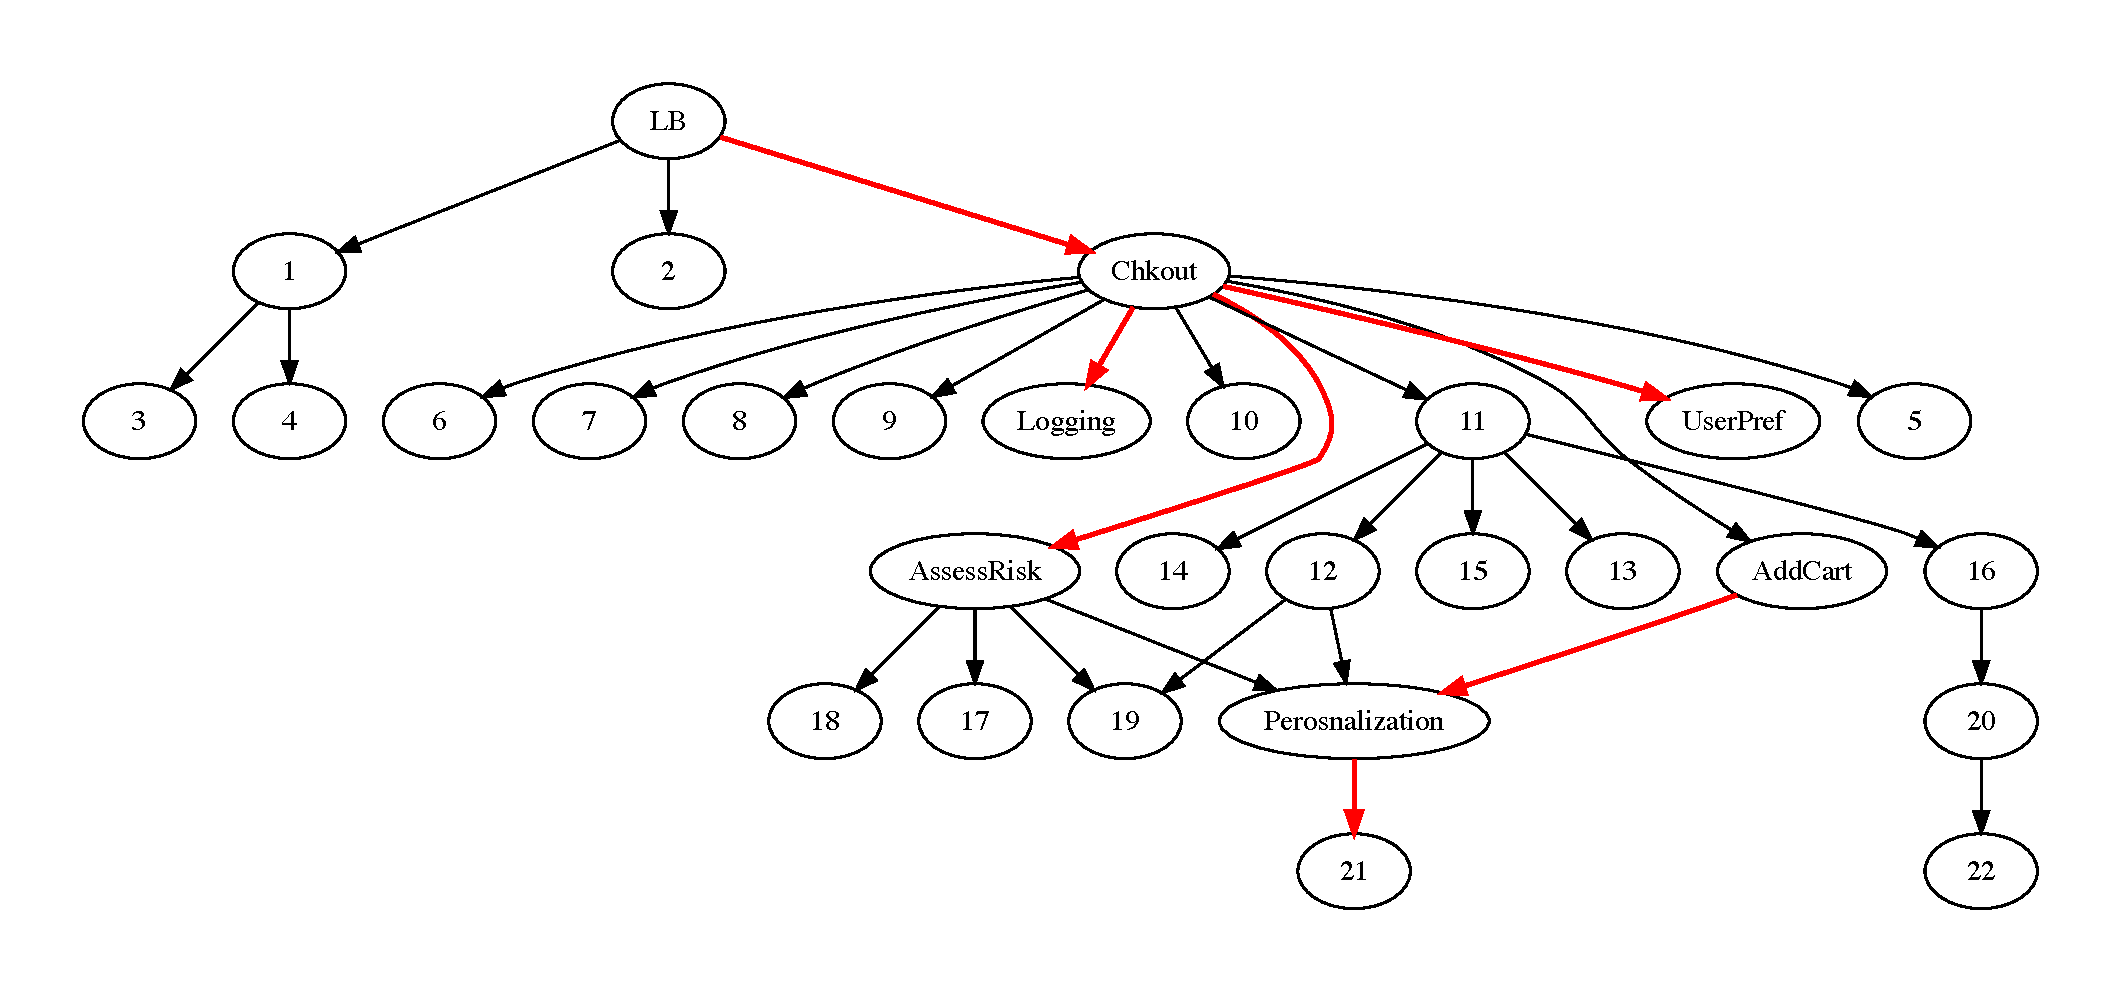
\includegraphics[scale=0.25]{anon_adrbk_fail.pdf}}
\caption{Example graph drawn from trace of a failed interaction. The red lines indicate that the callee has returned an error message to the caller}
\label{Failed_ex}
\end{figure}

To explain the triage process followed by site reliability engineers (SRE) when a failure occurs, we consider the example of a user trying to buy items from an online store. A successful checkout occurs when the user is able to place an order, else the checkout fails. Users being unable to checkout represents an outage of the system. Figure~\ref{Failed_ex} shows the  call-graph of a user interaction involving checkout of items for a cart during an outage. When users are unable to buy items form the store, it is the job of a site reliability engineer (SRE) to find out why. 
Currently, the SRE sees a number of alerts arising from failures, possibly in RPC calls highlighted as red in the call graph, from the monitoring system.  Subsequently, based on the alerts, the SRE may consult aggregate data such as error rates and latency over sliding windows of time for services deemed problematic.
The SRE might go about their job like so:
\begin{itemize}
\item Use domain knowledge about the dependencies between services to know which alerts are the result of transitive dependencies and must be ignored. \newline
As an example, the load balancer (LB) in the figure will be alerting as a result of its callee (Chkout) having returned an error message. This is indicated by the red line between LB and Chkout.  
An SRE with a good mental model of the system would conclude that since checkout (Chkout) has multiple downstream alerts, the alerts at LB are probably a result of the error being propagated up and try to dig deeper into one of the alerts from the downstream services. The reasoning is that a downstream service generating an alert is more likely to be a candidate for the proximal cause of the problem.  
\item Determine if the failure of some service(s) is the proximal cause \newline
Once a promising alert has been found, it is now time to look at the logs from the appropriate time to try to determine cause of failure. If the SRE determines service failure(s) to be proximal cause of the outage is caused by failure of mandatory services or a fallback path not being taken, she now has to \emph{obtain and compare} the trace of failed execution with that of one or more successful executions exercising the same request path. 
\end{itemize}

Both of the steps described above can be solved by comparing the trace of the failed execution with a family of successful traces in order to determine how the failed trace diverges from the successful traces. By witnessing a large number of successful executions during steady state, we can learn models from steady state data such that we construct representations for traces which encode the structural properties of the underlying graphs corresponding to the traces. Our technique for generating them derives from Word2Vec, which is used to generate word embeddings based on context of words in a sentence. Therefore, the trace representations learnt by our technique are called trace embeddings. Embeddings  serve two purposes:
\begin{enumerate}
\item Embeddings for traces can be classified before they are stored making it easy to find the most appropriate traces to compare to when a failure occurs.
\item As the number as well as the size of traces increase, storing the embeddings may be much more compact than the original traces. \kam{Since we haven't tried reversing our embedding to recapture the graphs, there may be some information loss here which we will need to quantify while making this claim. If we want to make this claim, that is}
\end{enumerate}

In the next section, we describe our technique for generation of trace embeddings and the corresponding distance measure used. In the evaluation, we describe how we use the fairly simple operations on the embeddings to address the problem described above and automatically generate hints about the proximal causes for the failure observed. 
%This is made possible by the fact that the embeddings encode information of structural neighborhoods.
%For outages which are not a result of service failures, a user entering invalid payment details perhaps or infrastructure failures, for example, appropriate next steps need to be taken. 